\documentclass{csfourzero}

\title{Too smart for your own good! A comparative evaluation of BERT and VADER sentiment analysis models under suboptimal conditions.}
\author{Arthur-Louis Heath}
\date{\today}
\usepackage{url}
\usepackage{natbib}
\usepackage{float}

\bibliographystyle{unsrt}

\abstract{The field of sentiment analysis studies techniques aimed at determining the sentiment of natural language text, a pursuit that is valuable for a variety of corporate applications. Current research is structured around a narrow set of standard benchmarks highlighting the strengths of complex deep learning models. This has created a disconnect between research and industry as many smaller actors do not have the computational or expert resources necessary to harness these in an applied context. This study addresses this deficiency by comparing representatives of the current state of the art in easy to implement rule-based approaches and sophisticated machine learning based ones. The Valence Aware Dictionary for Sentiment Reasoning rule-set and Bidirectional Encoder Representations from Transformers model recently made available by Google were found to be amongst the best performing in their respective classes of approach. The accuracy, precision, recall and $F_1$ scores of each were compared in a binary-sentiment classification problem structured to emulate messy real world conditions and resource scarcity. Google's model was found to be the superior of the two despite problem constraints, providing solid evidence for its dominance in a broader range of examples than the ones considered in prior research. }


\begin{document}
\maketitle


\section{Introduction}
\label{sec:intro}

The rapid expansion of the digital sales landscape is undoubtedly a hallmark of the 21st century. Social-media, e-commerce and crowd-sourced review platforms provide actors with large repositories of first-hand data on user experience. This data allows corporations to evaluate on a never-before-seen scale and facilitates improvements in their services, recommendation algorithms, quality control processes and more \cite{applications}. The challenge is, therefore, to develop techniques to extract useful information from this data, a research problem that the field of \textit{Sentiment Analysis} aims to address.
\par
The state-of-the-art in sentiment analysis consists mainly of deep learning based approaches able to detect complex features of natural language such as irony, word negation and the use of slang. Impressive results have been achieved, with deep learning based approaches outperforming non-ml based techniques on many popular benchmarks. Their performance, however, remains highly context dependant and is predicated on the availability of extensive, well-labelled data-sets. 
\par
Designing an approach to tackle sentiment analysis problem is a non-trivial issue. Comparative evaluation of disparate approaches to sentiment analysis across a wide range of possible scenarios is therefore required to help ease this overhead for both researchers and companies. We aim to contribute to this body of research through a study comparing the highly sophisticated BERT (Bidirectional Encoder Representations from Transformers) model \cite{BERT1} developed by Google to the ubiquitous rule-based model VADER (Valence Aware Dictionary for Sentiment Reasoning) \cite{vader}. Comparison will be conducted under challenging conditions simulating a class of problem currently underrepresented in the literature.

\section{Background and Related Work}
\label{sec:lit}
The field of sentiment analysis dates back to the early 2000s with the publication of
\cite{pangetal} and \cite{turneysemorientation}. There has been a sharp increase in interest since the early 2010s (explored in \cite{bibliometricssentimentanalysis}) due to the increased adoption of digital infrastructure and focus on user-generated content (some might call this the rise of Web 2.0). In addition to industrial applications, it has been successfully applied to a variety of problems, some interesting examples being stock price prediction \cite{smprediction} and political campaign management \cite{campaignprediction}.
\par
Sentiment analysis is primarily concerned with discerning the sentiment of pieces of natural language, although other metrics such as subjectivity may be of interest. Problems are classified according to the granularity of the desired classification \cite[Chapter 2.]{sentimentanalbook} and the level at which text is examined \cite{SAlevels}. In terms of the former, we differentiate between problems requiring the determination of opinion polarity ( negative/positive or negative/neutral/positive) and sentiment intensity.  In the latter, several categories representing a range of sentiments are created. Due to standard practices among online platforms, the 5-class (roughly corresponding to a 5-star rating) version is most common of these.
\par
According to the level at which text is examined, we differentiate between document level, feature level and sentence level approaches. At the document level, the entire text is considered as a single unit whereas, at the sentence level, fine-grained features pertaining to individual sentences are used.  Feature level sentiment analysis focuses on facets of a sentiment. A restaurant review for may, for example, express separate sentiments towards the food and service. Sentence level sentiment analysis is particularly popular since it is a more significant challenge and text instances in real-world data-sets are often short.
\par
Major challenges in sentiment analysis centre around the handling of complex natural language features such as irony and rhetorical questions \cite{challangesinSA}. The problem posed by these is most significant when individual data instances are small, informal and subjective. In an applied context, domain adaptation also poses a considerable challenge \cite{domainadaptation}. Due to the prevalence of machine learning approaches, the challenges faced by these also carry over.
\par
Many more established techniques for sentence-level sentiment analysis are Rule-Based. They work by quantifying the opinion held in individual words and applying a handcrafted set of rules to account for language features. A comprehensive study comparing these over a wide variety of data-sets and across a wide range of evaluation metrics has been preformed \cite{sentibench} and determined the VADER model to the best performing overall (its performance is depicted in Table \ref{tab:vaderPerf}).
\par

\begin{table}[h]
    \centering
    \begin{tabular}[t]{lccc}
        \hline
        Dataset & Problem & Accuracy \\
        \hline
        Tweets_RND_II & Polar & 99.04\% \\
        Tweets_STF & Polar & 84.44\% \\
        Comments_Digg & Polar & 69.05\% \\
        Comments_BBC & Polar & 62.76\% \\
        Tweets_Semeval & 3-class &  60.21\% \\
        Tweets_RND_III & 3-class & 60.14 \% \\
        Comments_BBC & 3-class &  49.40 \% \\
        Comments_NYT & 3-class & 48.03 \% \\
        \hline
    \end{tabular}
    \caption{Performance of VADER on Common Benchmarks \cite{sentibench}}
    \label{tab:vaderPerf}
\end{table}
    
\par
Several studies have attempted to characterise the state-of-the-art in machine learning approaches, notable examples are \cite{beneaththeiceberg} and \cite{stateOfTheArt}. Google's BERT was determined to be among the best performing models in both cases, with its variants placing among the top three across the examined set of benchmarks. BERT's performance in these studies is presented in Table \ref{tab:bertPerf}. 

\begin{table}[h]
    \centering
    \begin{tabular}[t]{lccc}
        \hline
        Dataset & Problem & Bert Variant & Accuracy \\
        \hline
        IMDB & Polar & BERT-large UDA & 95.8 \\
        Stanford Sentiment Treebank & 5-class & BERT-large & 55.5\% \\
        Stanford Sentiment Treebank & Polar & spanBERT & 94.8\% \\
        Semeval 2014 T4 SB2 & Aspect Level  & BERT-ADA & 84.0 \\
        \hline
    \end{tabular}
    \caption{Performance of BERT on Common Benchmarks \cite{beneaththeiceberg}}
    \label{tab:bertPerf}
\end{table}

Although there is no golden standard benchmark used in sentiment analysis, several have received disproportionate attention. Among others, these are the Stanford Sentiment Treebank \cite{SST}, IMDB Movie Reviews Data-set \cite{IMDB}, Paper Reviews Data Set and the OpinRank Review Data Set \cite{opinrank}. These are typically large and well labelled with the overwhelming majority containing data gathered from a single narrow domain. Many are also prepossessed to varying degrees. The purpose of this is to increase the proportion of `interesting` examples and unify attributes such as text length as in the example of the Stanford Sentiment Treebank.  

\par

There is no shortage of studies comparing various sentiment analysis techniques. Studies have been published evaluating state-of-the-art neural approaches to VADER \cite{lstmbertvader} and to compare traditional machine learning architectures to BERT \cite{mlcomp} \cite{bertml}, however, to the best of our knowledge no academic study directly compares the performance of the two. Research examining how a switch from benchmark to real-world conditions affects the performance of popular machine learning models is also scarce. Finally, research is often driven by the desire to compete on these benchmarks, meaning models are presented at their best. In the case of machine learning a large space of possible training and meta parameters is explored.

\section{Research Question}
\label{sec:rq}
Although sophisticated machine learning approaches to sentence-level sentiment analysis have the potential to achieve better performance, Rule-Based systems are ubiquitous and easy to implement. The former are also less robust, as they require large quantities of data and the non-trivial selection of parameters to achieve maximal results. Due to their comparative strengths and weaknesses, different scenarios favour one class of approach over another. Although much work has been done to compare them, this work is far from comprehensive as the range of possible scenarios and parameters is extremely broad. In addition to this, sentiment analysis is a fast-evolving subject with newer, more sophisticated options regularly becoming available. We propose a study comparing two wildly different, widely available state-of-the-art approaches. We will also aim to compare them in a scenario that is reflective of a difficult class of problem under-addressed in current literature. We hypothesize that in such scenarios, older, less sophisticated approaches may outperform machine learning based ones. To study this question, we will attempt to answer the following question:

\smallskip
\begin{center}
   \textbf{Can the VADER model out-preform BERT in binary sentiment analysis on a multi-domain dataset?}
\end{center}
\smallskip

Our secondary aims are to broaden understanding of the studied models and provide a solid base for future comparative research to build on. Additionally, our hope is this study might aid the decision making of smaller actors. 

\par
Broadly, design decisions taken aim to compare the best algorithms available in a challenging environment that might feasibly occur in the real-world. Both models selected are freely-available with VADER being practically ubiquitous due to its inclusion in the popular NLTK library \cite{nltk}. As previously discussed, they both also represent the pinnacle of their respective classes of approach in terms of benchmark performance.
\par

We have opted to use the unprocessed Multi Domain Sentiment Dataset (MDSD). This data-set contains Amazon product reviews distributed unevenly across various domains represented by product classes (listed in Appendix \ref{appendix:A}). Previous research into domain adaptation problems has shown there are significant structural differences between domains \cite{domainadaptation}. We therefore expect the MDSD to prove quite challenging. Such a data-set might be used in a scenario where a single domain data-set is unavailable (dataset augmentation). The informal nature and varying length of user-generated product reviews will present another challenge, as will the presence of complex natural language features.
\par
To compare BERT at its best, the base version of the model pre-trained on the BooksCorpus natural language corpus and English Wikipedia \cite{booksCorpus} will be used. Additional constraints will be introduced when fine-tuning BERT, namely, data scarcity will be simulated and default training parameters used. Such conditions are representative of limited access to data, computational resources and expert knowledge. 
\par
As the VADER model is rule-based and therefore does not require fine-tuning, it is expected to perform similarly regardless of these constraints, it may, however, be affected by the challenging nature of the MDSD dataset.

\par

Finally, accuracy is not always the best indicator of performance. In cases where false positives incur a high cost, such as when a company wishes to identify negative comments and respond to them, precision (\ref{eq:1}) is a preferable metric. Similarly, recall (\ref{eq:2}) may be preferred when identifying a high proportion of true positives is of the essence. 
\par

\begin{equation} \label{eq:1}
Precision = \frac{True\ Positives}{True\ Positives + False\ Positives}
\end{equation}

\begin{equation} \label{eq:2}
Recall = \frac{True\ Positives}{True\ Positives +  False\ Negatives}
\end{equation}

\par 
To this end we will consider a range of standard metrics in our comparison. Accuracy, precision, recall will all be compared along with $F_1$ scores (\ref{eq:3}) to evaluate the balance of precision and recall provided by each model. Finally, manual analysis of confusion matrixes will be conducted.
\begin{equation} \label{eq:3}
F_1 = \frac{2}{Recall^{-1} + Precision^{-1}}
\end{equation}

\section{Experimental Design}
\label{sec:exp}

\subsection{Hypothesis}

To answer our research question, we will attempt to prove the following hypothesis:

\begin{quote}
    \begin{center}
        \textbf{In the task of binary sentiment classification on subsets of the MDSD dataset VADER will significantly outperform BERT in either Accuracy, Precision, Recall or $F_1$ score when the latter is trained on limited training data (12500 instances) using default parameters.}
    \end{center}
\end{quote}

Should we confirm this hypothesis, we will have proved the existence of a class of (real world) scenario where actors might preferentially choose a rule-based approach to a sophisticated ML-based one and will answered our research question.

\subsection{Dataset}

To prepare datasets for binary classification, the MDSD was first prepossessed as in \cite{domainadaptation}. The bodies of reviews assigned 1 or 2 stars were assigned the 'negative' label and ones with 4 or 5 stars the 'positive' one. Ambiguous reviews (3 stars) were discarded.
\par
In total, 30 balanced subsets of 10000 randomly selected reviews were constructed. Each of these was assigned a non-overlapping set of 12500 reviews to serve as fine-tuning data for BERT. In Machine Learning, the 70-20-10 and similar rule-of-thumb ratios of training, validation and test datasets are common \cite{testvalsplit}, using 12500 reviews for training and validation is therefore roughly analogous to a situation with approximately 15000 total reviews available. This is several orders of magnitude smaller than the datasets examined in Section \ref{sec:lit} and is small compared to the number of BERT's trainable parameters (approx. $1.1 \times 10^8$). The size of training dataset, therefore represents a scenario of radical data scarcity. The decision to use balanced datasets was made to increase applicability, as the label distribution in product reviews is specific and does not translate to other domains \cite{jshapedreviews}.

\subsection{Materials}

Both models were adapted to serve as binary sentiment classifiers. In the case of BERT, the Pre-Trained uncased version of the BERT-Base model was sourced via google's API \cite{bertavailable}. An additional super-dense layer consisting of 2 nodes with Softmax activation functions was connected to the final NSP-Dense (next sentence prediction) layer of the model. The output of this layer served as a one-hot encoding of the classification space. This manner of adaptation is precedented in the literature in \cite{bertAdaptation}.
\par
The version of VADER distributed with the popular NLTK library (Version 3.5) \cite{NLTKoriginalpaper} was used. VADER outputs a compound sentiment score in the range $(-1,\ 1)$. The signum of this score represents a 'positive' or 'negative' classification label. Scores of 0.0 (indeterminable sentiment) were randomly assigned to allow for comparison with BERT while avoiding the introduction of a persistent bias, 
\par
The full implementation of testing code is available at \cite{GITBUB}. Training was performed on in a freely available Google Colaboratory environment. Software packages used, versions and hardware specifications are included in Appendix \ref{appendix:B}

\subsection{Population and Sampling}

BERT and VADER were applied to each dataset in turn, and the results used to create eight samples (one for each metric for each model). Fine-tuning of BERT was performed separately for each dataset, as this avoided the risk of examining an unrepresentative version of BERT (statistical outlier). Default training parameters were sourced from the original paper\cite{BERT1} and are listed in \ref{tab:trainingParameters}.

\par
\begin{table}[ht]
    \centering
    \begin{tabular}[t]{lcc}
        \hline
        Parameter & Value \\
        \hline
        Training Size & 10,000 \\
        Validation Size & 2,500 \\
        Train-Val Split  & 80\%-20\% \\
        Sequence Length & 128 \\
        Batch Size & 16 \\
        Num. Epochs & 3 \\
        Learning Rate & $2 \times 10^{-5}$
        \hline
    \end{tabular}
    \caption{Fine-Tuning (Training) Parameters for BERT Model}
    \label{tab:trainingParameters}
\end{table}
\par

\subsection{Statistical Testing}

\par
\begin{figure}[h]
    \centering
    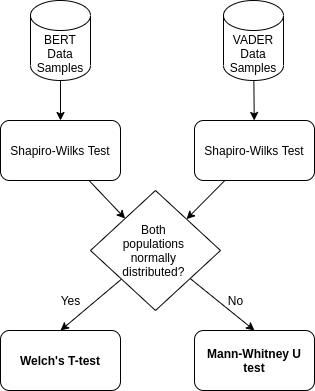
\includegraphics[width=0.5\textwidth]{img/statistical_tests.png}
    \caption{Strategy for statistical tests.}
    \label{fig:statstrat}
\end{figure}
\par

In addition to direct analysis of the samples, a suite of statistical tests was devised to generalise results to all possible comparisons in the scenario context (population space) and to attempt to establish the stochastic dominance of one model over the other. The procedure depicted in Figure \ref{fig:statstrat} was applied to pairs of samples (one of BERT and one of VADER) in turn for each considered metric. In all instances a significance threshold of 5\% ( $\alpha=0.05$) was used.
\par
For each individual sample, a Shapiro-Wilks normality test was first performed under the following null and alternate hypotheses:
\par
\begin{quote}[H]
    \begin{center}
        \begin{itemize}
            \item\textit{$H_0$ The sample is sourced from a normally distributed population.}
            \item\textit{$H_{0}^A$ The sample is sourced from a non-normal distribution.}
        \end{itemize}
    \end{center}
\end{quote}
\par

For each pair of samples corresponding to a given metric, if $H_0$ had been rejected for either population, a Mann-Whitney U test was performed on the following hypotheses with A representing the population with the greater mean:

\par
\begin{quote}
    \begin{center}
        \begin{itemize}
            \item\textit{$H_{1}$ Population A is stochastically equal to population B.}
            \item\textit{$H_{1}^{A}$ Population A is stochastically greater than population B.}
        \end{itemize}
    \end{center}
\end{quote}
\par

The Mann-Whitney U test is appropriate here as it is considered to be better as it does not assume the distributions are normal, however, it carries assumptions about the similarity of the distribution's shapes that might weaken results \cite{mannwhitneyU}. Use of Welch's T-test is therefore preferable in cases where both distributions are normal. To this end, if $H_{0}$ was confirmed for both samples, Welch's T-Test was used for under the same hypotheses. Note that Welch's T-test is performed regardless of homogeneity of variances; this was done in line with the emerging consensus in the literature \cite{welchgood1}\cite{welchgood2}.

%Guide length: 500 words.
\section{Results}
\label{sec:results}

\par
Figures \ref{fig:bertcmat} and \ref{fig:vadercmat} depict the average-case confusion matrices for both models. They were created by summing the classification results of each experiment run and normalizing the resulting matrix. 
\par
\begin{figure}[H]
    \centering
    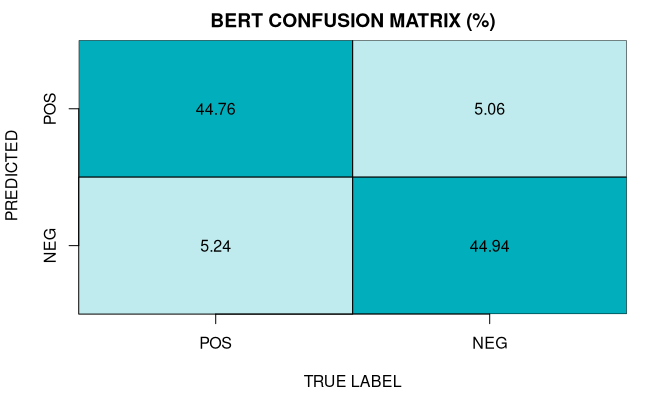
\includegraphics[width=0.8\textwidth]{img/bert_cmat_plot.png}
    \caption{Normalised Mean Confusion Matrix of BERT}
    \label{fig:bertcmat}
\end{figure}
\par

The confusion matrix of BERT (Figure \ref{fig:bertcmat}) demonstrates appears to be balanced and the model did not demonstrate a preference for either label. Note that this result may not generalise to heavily unbalanced datasets due to the so called `accuracy paradox` \cite{ACCURACYPARADOX}.
\par
\begin{figure}[H]
    \centering
    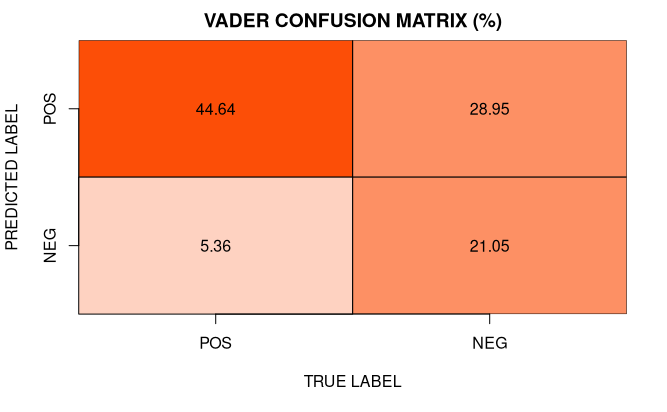
\includegraphics[width=0.8\textwidth]{img/vader_cmat_plot.png}
    \caption{Normalised Mean Confusion Matrix of VADER}
    \label{fig:vadercmat}
\end{figure}

\par
The confusion matrix of VADER (\ref{fig:vadercmat}) appears highly unbalanced despite its success classifying positive review instances. Its classification of negative instances was far less successful, with false positives occurring 37.52\% more frequently than true negatives. This may be indicative of an overall tendency towards assigning positive labels, or difficulties in correctly identifying negative sentiment. The latter case could be due to irregularities in either the lexicon itself or the underlying data.
\par

\begin{figure}[H]
    \centering
    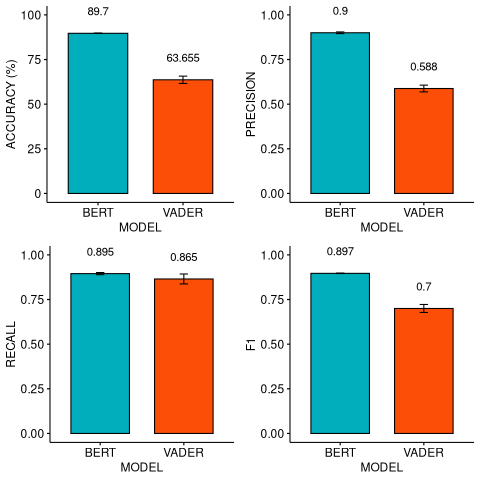
\includegraphics[width=0.8\textwidth]{img/metric_charts.png}
    \caption{Comparison of BERT/VADER Metric Performance}
    \label{fig:metriccharts}
\end{figure}

\par
The mean performance of both models in each of the considered metrics is presented in Figure \ref{fig:metriccharts}. BERT appears to have dominated in accuracy and precision. While both models attained a similar rate of recall, the mean performance of BERT was still higher by 3.4\%. Considering its dominance in recall and precision, it is unsurprising that BERT also achieved a higher mean $F_1$ score. In the three non-composite metrics (accuracy, precision and recall) BERT outperformed VADER by an average of 32.45\%.
\par

\subsection{Statistical Tests}

As per the planned testing strategy (Figure \ref{fig:statstrat}), the Shapiro-Wilks normality test was first performed on the populations (each metric for each model) to attempt to prove they were sampled from normal distributions. The results of these tests are presented in Table \ref{tab:swresults}, with a p-value smaller than the threshold ($\alpha = 0.05)$ serving as grounds to reject REFERNECENULLHYPOTHESIS meaning that the samples parent distribution is statistically unlikely to be normal. A p-value above the threshold, therefore provides evidence that the parent distribution is in fact, normal.

\begin{table}[H]
    \centering
    \caption{Shapiro-Wilks Test Results}
    \begin{tabular}[t]{lccccc}
        \hline
            Metric & BERT Statistic &  BERT Sig. & VADER Statistic & VADER Sig.\\
        \hline
            Accuracy & 0.855 & $8.01 \times 10^{-4}$ & 0.975 & 0.707 \\
            Precision & 0.969 & 0.534 & 0.971 & 0.591 \\
            Recall & 0.979 & 0.810 & 0.955 & 0.233\\
            $F_1$ Score &0.787 & $3.89 \times 10^{-5}$  & 0.970 & 0.531\\
        \hline
    \end{tabular}
    \label{tab:swresults}
\end{table}

\par

The majority of test samples (including all of those generated by VADER) were determined to come from normally distributed populations. The exceptions were the populations corresponding the accuracy and $F_1$ score of BERT (p-value under 0.05). The structure of these is presented in greater detail in \ref{fig:wierddist}. 

\begin{figure}[H]
    \centering
    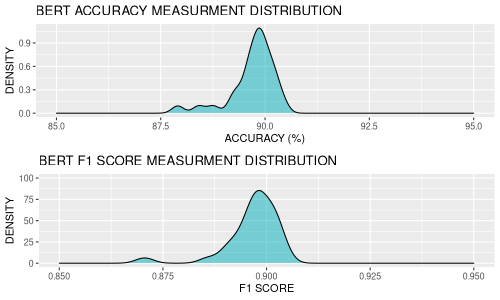
\includegraphics[width=0.9\textwidth]{img/odd_distributions.png}
    \caption{Comparison of BERT/VADER Metric Performance}
    \label{fig:wierddist}
\end{figure}

\par 
Both distributions appear to be negatively skewed and contain several negative outliers. This may be a consequence of BERT's need for fine-tuning (the key difference between the two). This result might mean that in rare cases, pre-training of BERT might generate a significantly inferior model, and vindicates the decision to perform pre-training for each dataset separately. However, even these outliers have outperformed VADER by a large margin and are therefore unlikely to affect a comparison.

\par

In line with the stated testing strategy, recall and performance were compared using Welch's T-test (Table \ref{tab:indiettest}) and accuracy and $F_1$ scores using the Mann-Whitney U test (Table \ref{tab:mannwhitney}).

\begin{table}[H]
    \centering
    \caption{Welch's T-Test Results}
    \begin{tabular}[t]{lcc}
        \hline
            Metric & T Statistic & Significance \\
        \hline
        Precision & 0.376 & $1.74 \times 10^{-54} $  \\
        Recall & 0.376 & $0.708$ \\
        \hline
    \end{tabular}
    \label{tab:indiettest}
\end{table}

\par

In the case of recall, the test failed to reject the null hypothesis, and we were, therefore, unable to establish a statistically significant result. For precision, however, BERT was shown to be stochastically dominant. Similarly, the Mann-Whitney U test results show the dominance of BERT in accuracy and $F1$ scores in line with the differences observed in the samples.


\begin{table}[H]
    \centering
    \caption{Mann-Whitney U Test Results}
    \begin{tabular}[t]{lcc}
        \hline
            Metric & U Statistic & Significance \\
        \hline
        Accuracy & 900.0 & $1.43 \times 10^{-11} $  \\
        $F_1$ Score & 900.0 & $1.44 \times 10^{-11} $ \\
        \hline
    \end{tabular}
    \label{tab:mannwhitney}
\end{table}


\section{Discussion}
\label{sec:discuss}

Statistical testing has proven that in the examined scenario, BERT outperforms VADER by a significant margin in three of four metrics and performs similarly in the fourth. It is, therefore, safe to say that regardless of the priority assigned to each metric, BERT has outperformed VADER and our stated hypothesis if false.
\par
Despite failing to confirm our research question, the results do not prove it to be false in general, as VADER might still outperform BERT in some other scenario. This could be achieved by tightening existing constraints or by introducing new confounding factors. For example, a heavily unbalanced training dataset or difference in training and test domain distributions (domain adaptation) might also serve to narrow the gap.
\par
The result is likely due in part to the quality of pre-training performed by Google Research. It indicates that the availability of pre-training data has a relatively small impact on BERT's overall performance. The significance of a multi-domain dataset is also called into question, as this would imply that few features of the language are learned during fine tuning. The discrepancy in performance may also be due to VADER performing badly (evidenced by the unbalanced confusion matrix). It is possible that this is due to the chosen classification threshold (although this is the one chosen by its creators), and could be explored by looking at its ROC curve. However depending on what effect is at play, altering this may have a symmetric effect on negative and positive classification and harm it's comparatively high recall. VADER was also created to classify social media posts. Although the literature indicates that this translates well to user generated data in general, it is always possible that product reviews in particular are an exception. To avoid post-hoc experimentation confirmation of these claims is left to future work.

\section{Conclusion \& Future Work}
\label{sec:conc}

Despite being negative, our findings still hold considerable value in the context of our secondary aims outlined in \ref{sec:rq}. We have shown that despite significant constraints machine learning models like BERT can achieve impressive results. By using default training parameters, a small number of epochs and freely available computational resources (Google Colaboratory), we have also demonstrated that such results are feasibly attainable by small actors. These may still wish to consider state-of-the-art models, even without access to the expert resources needed to optimise them fully. Finally, as the examined scenario is an uncommon one, we have enriched the existing body of research by demonstrating that BERT's value might also lie outside of the idealised scenarios of popular benchmarks. 

\par
A limitation of this study is the arbitrary nature of the examined scenario. Further experiments will be performed to model the effect individual factors have on BERT's performance. This would enable researchers to make an informed guess as to what parameters might tip the balance in VADER's favour and prevent the further expenditure of resources on negative studies such as this one. The final aim of such research would be the construction of a general predictive framework of BERT and VADER performance. Although we have justified the choice of scenario used, examining a concrete real-world scenario faced by a specific company could increase applicability and help to ground the results. Finally, the choice of metrics in this study is far from comprehensive and could be expanded by a future study.


\section{Reflective Analysis}

My original plan for this study turned out to be overambitious both in terms of the resources I had available and the space in this report. This is something that became apparent to me late into the project, and consequently, a lot of my early work was discarded. Although this mistake was partly due to my inexperience in the field but could have been averted through better preparation and paying closer attention to the lecture on statistical tests. Additionally, I greatly underestimated the performance of BERT. If I had the chance to design this study again, I would spend more time predicting the models' performance to decrease the likelihood of a negative result.
\par
Overall I found the project to be highly enjoyable to work on, as I am seldom given a chance to dive into a topic `head-first` as part of my other courses. Experimenting with the state-of-the-art in machine learning was also rewarding, and I was greatly impressed with the performance of BERT.


\bibliography{myrefs}
\newpage

\appendix

\section{Domain Structure of the Multy Domain Sentiment Dataset}
\label{appendix:A}

\begin{table}[H]
    \centering
    \begin{tabular}[t]{lc}
        \hline
        Category & Number of Reviews \\
        \hline
        apparel & 	7252 \\
        automotive & 	654 \\
        baby & 	2356 \\
        beauty & 	1391 \\
        books & 	973194 \\
        camera \& photo & 	5409 \\
        cell phones \& service &  1113 \\
        computer \& video games & 	1313 \\
        dvd & 	122438 \\
        electronics & 	21009 \\
        gourmet food & 	367 \\
        grocery & 	1280 \\
        health \& personal care & 	5225 \\
        jewelry \& watches & 	689 \\
        kitchen \& housewares & 	17856 \\
        magazines & 	2221 \\
        music & 	172180 \\
        musical instruments & 	308 \\
        office products &	431 \\
        outdoor living & 	272 \\
        software & 475 \\
        sports \& outdoors & 	3728 \\
        tools \& hardware & 	112 \\
        toys \& games & 	11147 \\
        \hline
    \end{tabular}
    \caption{Domain Distribution in MDSD dataset \cite{sentibench}}
    \label{tab:vaderPerf}
\end{table}

\newpage

\section{Hardware and Dependency Details}
\label{appendix:B}

\subsection{Hardware Details for BERT Training and Testing}

Regret ably, Google Collaborative does not make the details of their hardware easily accessible, the following is as exhaustive a list as could be compiled.

\begin{verbatim}
processor : 0
vendor_id : GenuineIntel
cpu family : 6
model  : 63
model name : Intel(R) Xeon(R) CPU @ 2.30GHz
cpu MHz  : 2300.000
cache size : 46080 KB
GPU name: Tesla K80
GPU compute capability: 3.7
MemTotal:       13333596 kB

\end{verbatim}

\subsection{Hardware Details for Other Experiments and Analysis}

\begin{verbatim}
H/W path           Device          Class          Description
=============================================================
                                   system         20JNS0V801 (LENOVO_MT_20JN_BU_Think_FM_ThinkPad T470 W10DG)
/0                                 bus            20JNS0V801
/0/3                               memory         16GiB System Memory
/0/3/0                             memory         16GiB SODIMM DDR4 Synchronous Unbuffered (Unregistered) 2133 MHz (0.5 ns)
/0/3/1                             memory         [empty]
/0/7                               memory         128KiB L1 cache
/0/8                               memory         512KiB L2 cache
/0/9                               memory         4MiB L3 cache
/0/a                               processor      Intel(R) Core(TM) i7-6600U CPU @ 2.60GHz
/0/b                               memory         128KiB BIOS
/0/100                             bridge         Xeon E3-1200 v5/E3-1500 v5/6th Gen Core Processor Host Bridge/DRAM Registers
/0/100/2                           display        Skylake GT2 [HD Graphics 520]
/0/100/14                          bus            Sunrise Point-LP USB 3.0 xHCI Controller
/0/100/14/0        usb1            bus            xHCI Host Controller
/0/100/14/0/2                      input          Razer DeathAdder
/0/100/14/0/4                      input          USB Keyboard
/0/100/14/0/7                      communication  Bluetooth wireless interface
/0/100/14/0/8                      multimedia     Integrated Camera
/0/100/14/0/9                      generic        Generic USB device
/0/100/14/1        usb2            bus            xHCI Host Controller
/0/100/14/1/3                      storage        USB3.0-CRW
\end{verbatim}


\subsection{R Evironment}
\begin{verbatim}
R version 4.0.3 (2020-10-10)
Platform: x86_64-pc-linux-gnu (64-bit)
Running under: Arch Linux

Matrix products: default
BLAS:   /usr/lib/libblas.so.3.9.0
LAPACK: /usr/lib/liblapack.so.3.9.0

locale:
 [1] LC_CTYPE=en_US.UTF-8       LC_NUMERIC=C               LC_TIME=en_US.UTF-8        LC_COLLATE=en_US.UTF-8     LC_MONETARY=en_US.UTF-8   
 [6] LC_MESSAGES=en_US.UTF-8    LC_PAPER=en_US.UTF-8       LC_NAME=C                  LC_ADDRESS=C               LC_TELEPHONE=C            
[11] LC_MEASUREMENT=en_US.UTF-8 LC_IDENTIFICATION=C       

attached base packages:
[1] stats     graphics  grDevices utils     datasets  methods   base     

other attached packages:
 [1] plot.matrix_1.5.2 ggpubr_0.4.0      readxl_1.3.1      forcats_0.5.0     stringr_1.4.0     dplyr_1.0.2       purrr_0.3.4      
 [8] readr_1.4.0       tidyr_1.1.2       tibble_3.0.4      ggplot2_3.3.2     tidyverse_1.3.0  

loaded via a namespace (and not attached):
 [1] tidyselect_1.1.0  xfun_0.19         haven_2.3.1       carData_3.0-4     colorspace_2.0-0  vctrs_0.3.5       generics_0.1.0   
 [8] htmltools_0.5.0   yaml_2.2.1        rlang_0.4.8       pillar_1.4.7      foreign_0.8-80    glue_1.4.2        withr_2.3.0      
[15] DBI_1.1.0         dbplyr_2.0.0      modelr_0.1.8      lifecycle_0.2.0   munsell_0.5.0     ggsignif_0.6.0    gtable_0.3.0     
[22] cellranger_1.1.0  zip_2.1.1         rvest_0.3.6       evaluate_0.14     rio_0.5.16        knitr_1.30        curl_4.3         
[29] fansi_0.4.1       broom_0.7.2       Rcpp_1.0.5        scales_1.1.1      backports_1.2.0   jsonlite_1.7.1    abind_1.4-5      
[36] fs_1.5.0          hms_0.5.3         digest_0.6.27     openxlsx_4.2.3    stringi_1.5.3     rstatix_0.6.0     grid_4.0.3       
[43] cli_2.2.0         tools_4.0.3       magrittr_2.0.1    crayon_1.3.4      car_3.0-10        pkgconfig_2.0.3   ellipsis_0.3.1   
[50] data.table_1.13.2 xml2_1.3.2        reprex_0.3.0      lubridate_1.7.9.2 assertthat_0.2.1  rmarkdown_2.5     httr_1.4.2       
[57] rstudioapi_0.13   R6_2.5.0          compiler_4.0.3   
\end{verbatim}


\subsection{Python Environment}
\begin{verbatim}
Package                Version   
---------------------- ----------
absl-py                0.11.0    
astunparse             1.6.3     
beautifulsoup4         4.9.3     
cachetools             4.1.1     
certifi                2020.11.8 
chardet                3.0.4     
click                  7.1.2     
cycler                 0.10.0    
gast                   0.3.3     
google-auth            1.23.0    
google-auth-oauthlib   0.4.2     
google-pasta           0.2.0     
grpcio                 1.33.2    
h5py                   2.10.0    
idna                   2.10      
joblib                 0.17.0    
Keras-Preprocessing    1.1.2     
kiwisolver             1.3.1     
lxml                   4.6.1     
Markdown               3.3.3     
matplotlib             3.3.3     
nltk                   3.5       
numpy                  1.18.5    
oauthlib               3.1.0     
opt-einsum             3.3.0     
pandas                 1.1.4     
Pillow                 8.0.1     
pip                    20.0.2    
protobuf               3.14.0    
pyasn1                 0.4.8     
pyasn1-modules         0.2.8     
pyparsing              2.4.7     
python-dateutil        2.8.1     
pytz                   2020.4    
regex                  2020.11.13
requests               2.25.0    
requests-oauthlib      1.3.0     
rsa                    4.6       
scikit-learn           0.23.2    
scipy                  1.5.4     
setuptools             46.0.0    
six                    1.15.0    
sklearn                0.0       
soupsieve              2.0.1     
tensorboard            2.4.0     
tensorboard-plugin-wit 1.7.0     
tensorflow             2.3.1     
tensorflow-estimator   2.3.0     
termcolor              1.1.0     
threadpoolctl          2.1.0     
tqdm                   4.52.0    
urllib3                1.26.2    
Werkzeug               1.0.1     
wheel                  0.34.2    
wrapt                  1.12.1    
\end{verbatim}
\end{document}
